% ----------------------------------------------------------------------

\chapter{\textbf{Objeções}} % Este comando é utilizado para criar capítulos

Durante a elaboração deste trabalho, foi constatado uma objeção, o tamanho dos modelos em relação a quantidade de dados utilizados na etapa de treinamento. \par
Os modelos de machine learning geralmente possuem crescimento logarítmico em relação a entrada de dados, ou seja, a partir de certa quantidade de dados processados, o espaço gasto para alocar os modelos tendem a se estabilizar em uma curva logarítmica. O mesmo fenômeno também pode ser observado durante a comparação de performance do modelo versus a quantidade de dados utilizados no treinamento.\par

\begin{figure}[h!]
	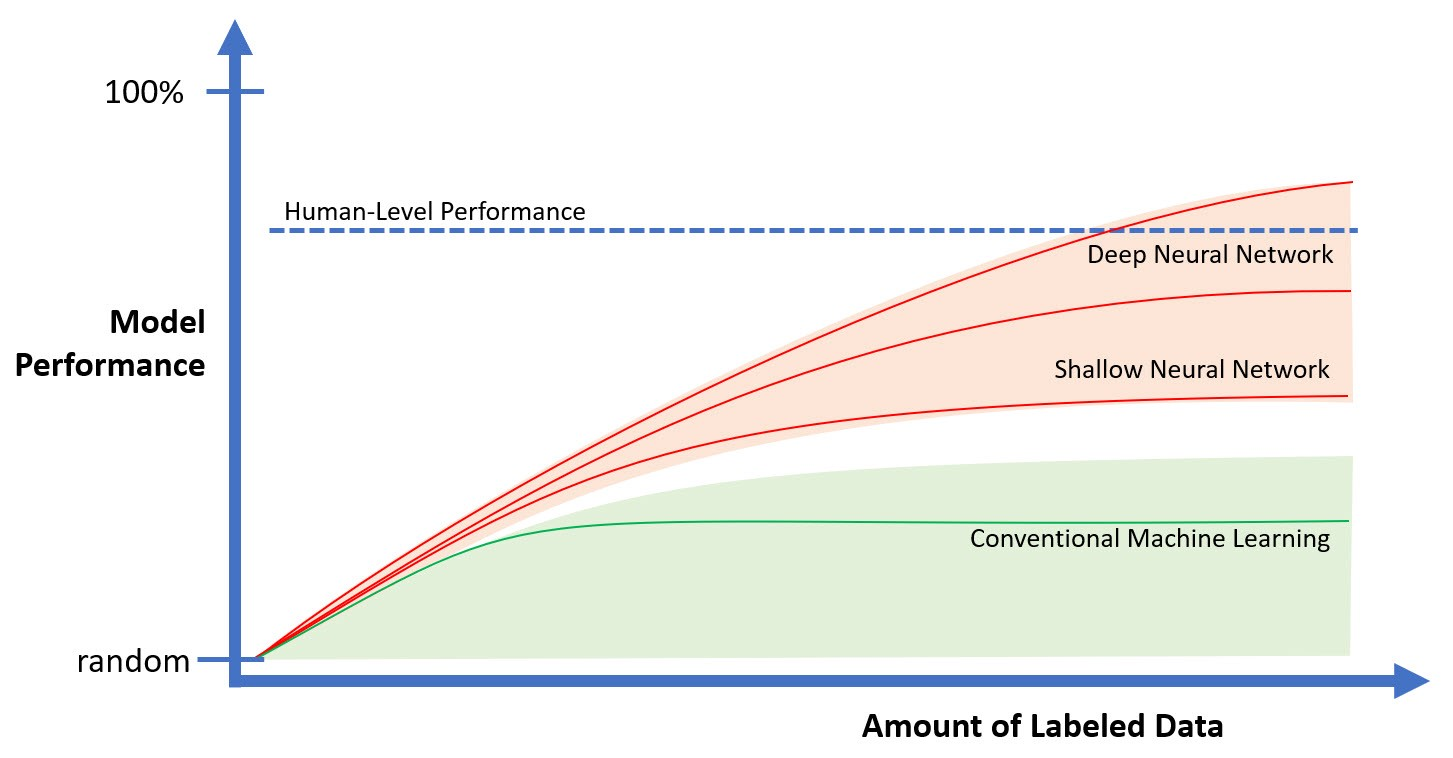
\includegraphics[width=\linewidth]{topics/dataperform.jpeg}
	\caption{Comparativo entre quantidade de dados versus performance generalista do modelo, por \cite{Hackathorn2018}.}
	\label{fig:dataperformgraph}
\end{figure}

Com os estudos realizados durante a produção deste trabalho, constatamos que a ideia de resolver o problema de distribuição dos modelos de machine learning não parece ser a melhor forma de solucionar esse problema específico. Para isso, existem outros tipos de otimizações a serem feitas que reduzem o tamanho de funções desse modelo, podendo ser reduzido em espaço e contendo performance compatível ou superior a modelos mais otimizados. \par
A definição dos modelos como uma curva logarítmica foi crucial, pois com essa definição foi possível constatar que no início dos testes e treinamento o modelo geralmente vai se comportar de forma crescente, mas tente a se estabilizar em decorrer do aumento dos dados, por isso, torna a questão como solucionada e não tendo a necessidade desse tipo de projeto para a possível solução a curto prazo de uma modelagem com falta de otimização.\par
